\setlength{\tabcolsep}{1pt}
\begin{figure}[h]
    \footnotesize
    \begin{tabularx}{\columnwidth}{ *{6}{Y} }
        Input & \ptopzero &  \nulltext &  \directinversion &  \negprox &  \method \\
        \multicolumn{6}{c}{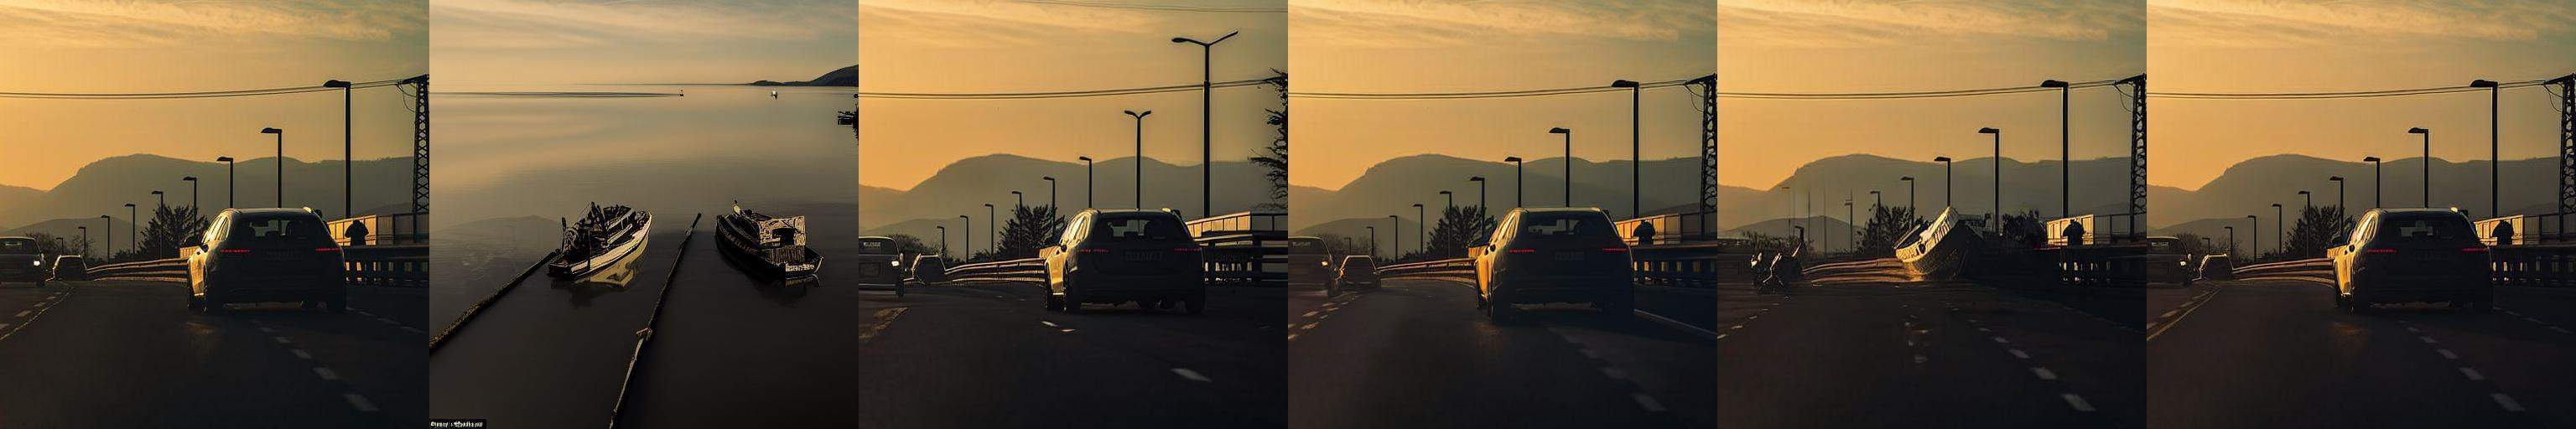
\includegraphics[width=\linewidth]{fig/ex_fail/all/1_change_object_80-2_natural-4_outdoor-124000000000}} \\
        \multicolumn{6}{c}{``\textit{\textcolor{BrickRed}{\st{cars}} \textcolor{RoyalBlue}{\textbf{boats}} driving on a highway at sunset}"} \\
        \multicolumn{6}{c}{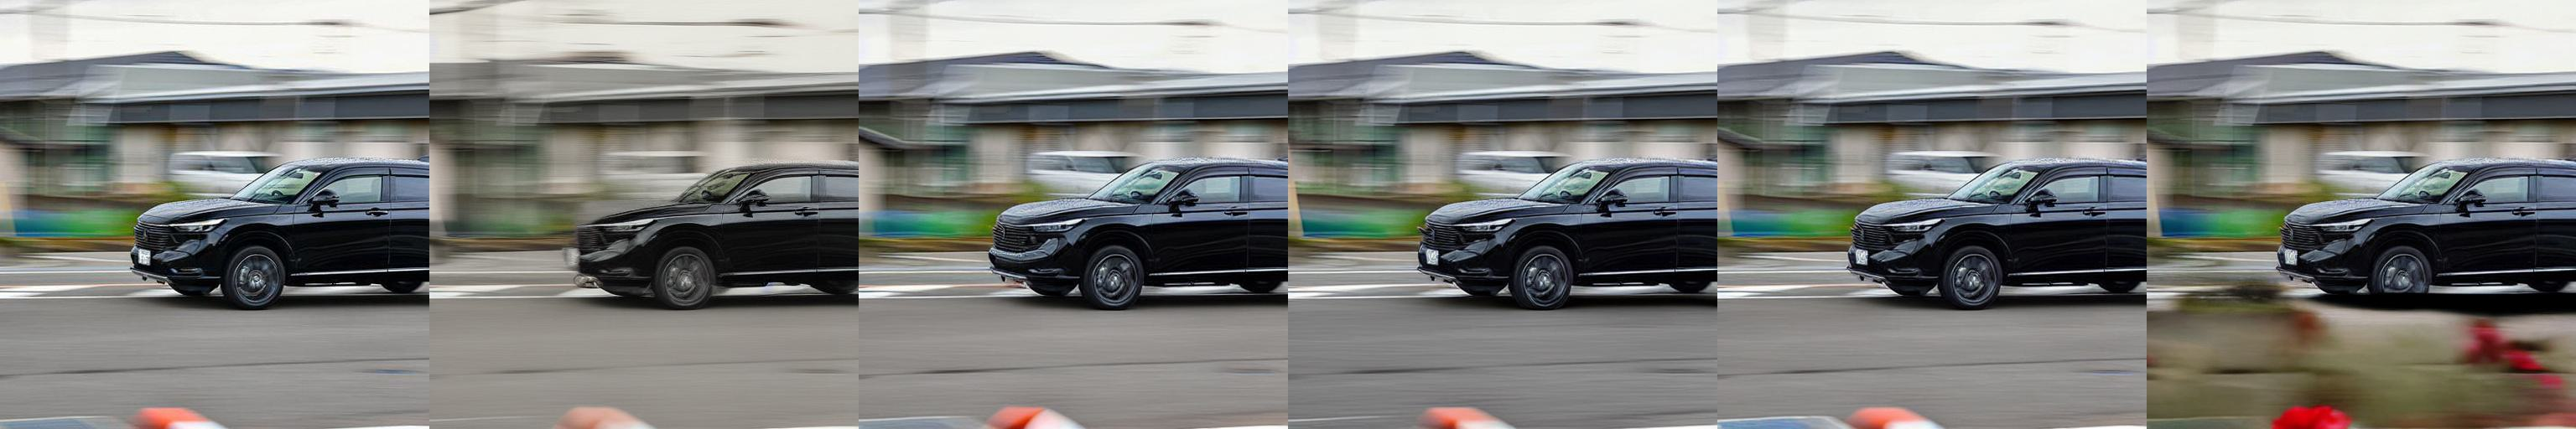
\includegraphics[width=\linewidth]{fig/ex_fail/all/7_change_attribute_material_40-2_natural-4_outdoor-724000000002}} \\
        \multicolumn{6}{c}{``\textit{the 2020 honda hrx is driving down the road \textcolor{RoyalBlue}{\textbf{full of flowers}}}"} \\
        \multicolumn{6}{c}{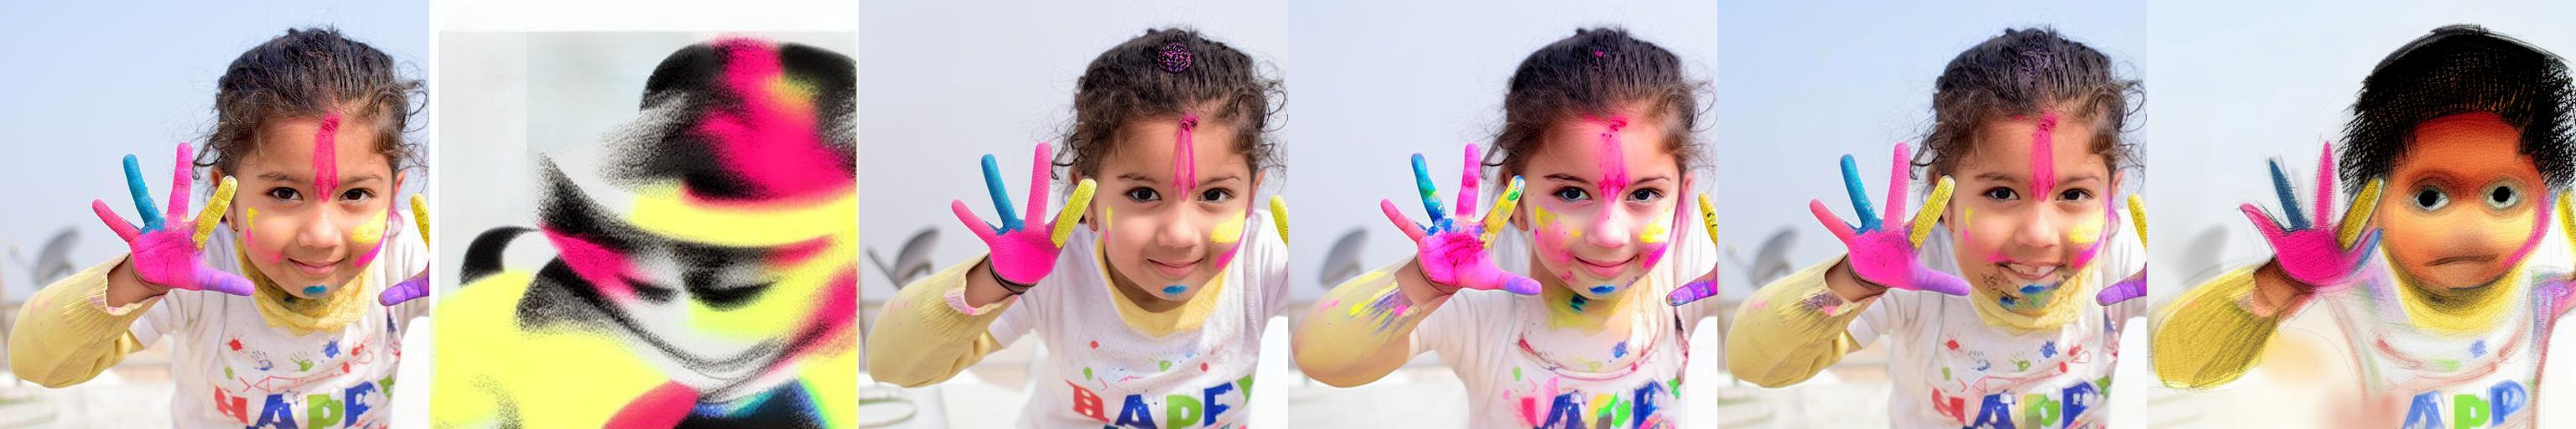
\includegraphics[width=\linewidth]{fig/ex_fail/all/9_change_style_80-2_natural-2_human-922000000009}} \\
        \multicolumn{6}{c}{``\textit{\textcolor{RoyalBlue}{\textbf{black and white sketch of}} a young girl with painted hands and face}"} \\
        \multicolumn{6}{c}{
\includegraphics[width=\linewidth]{fig/ex_fail/us/7_change_attribute_material_40-1_artificial-1_animal-711000000004}} \\
        \multicolumn{6}{c}{``\textit{a kitten \textcolor{RoyalBlue}{\textbf{sculpture}} }"} \\
        \multicolumn{6}{c}{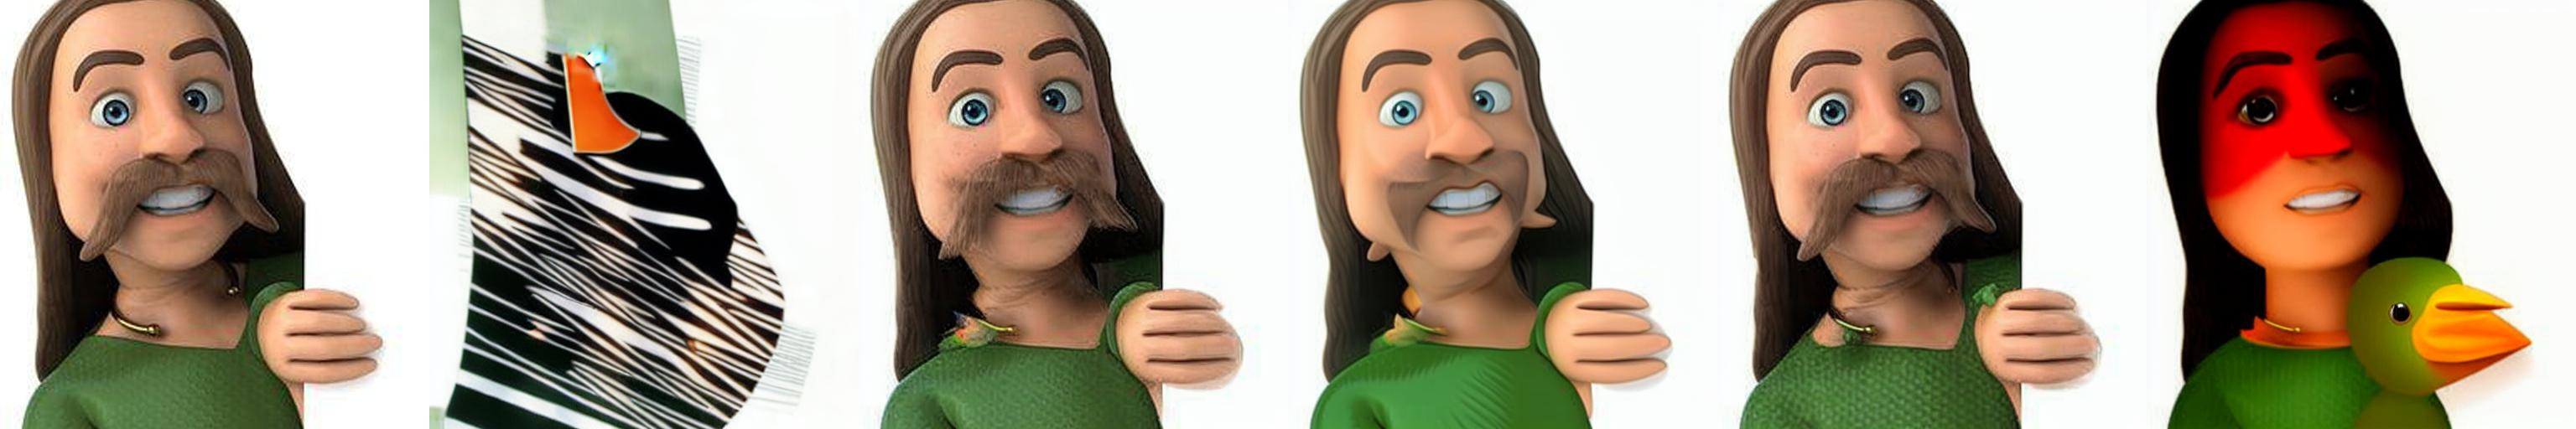
\includegraphics[width=\linewidth]{fig/ex_fail/satur/2_add_object_80-1_artificial-2_human-212000000008}} \\
        \multicolumn{6}{c}{``\textit{a cartoon man \textcolor{RoyalBlue}{\textbf{and a bird}}}"} \\
        \end{tabularx}
        \caption{This figure presents examples from the PieBench dataset where various methods, including ours, encounter difficulties in achieving the desired editing outcomes. These images highlight the challenges and limitations faced in specific editing scenarios, providing insights into areas where each method may require further refinement or adaptation.}
        % \caption{Examples from the PieBench dataset highlighting failure cases across different methods. The figure shows scenarios where the intended edits are not achieved due to the sensitivity of CFG-based approaches to hyperparameter choices. In rare instances, SAGE produces oversaturated and poorly reconstructed images—issues that can be alleviated by reducing the CFG weight ($w$) and self-attention guidance ($\lambda$).}
    \label{fig:sup_exfailall}
  \end{figure} 